\chapter{Evaluation of methods}
\label{sec:evaluation}

\begin{listing}
\begin{hminted}
let f : Int /\rar/ Int =
  /\lbd/ x . {
    case x of
    | 0 /\Rar/ 0
    | 1 /\Rar/ 1
    | n /\Rar/ f (n - 1) + f (n - 2)
    end
  }
in f 25  
\end{hminted}
\caption{An evaluation-heavy Hazel program with no holes}
\end{listing}

\begin{figure}
  \centering
  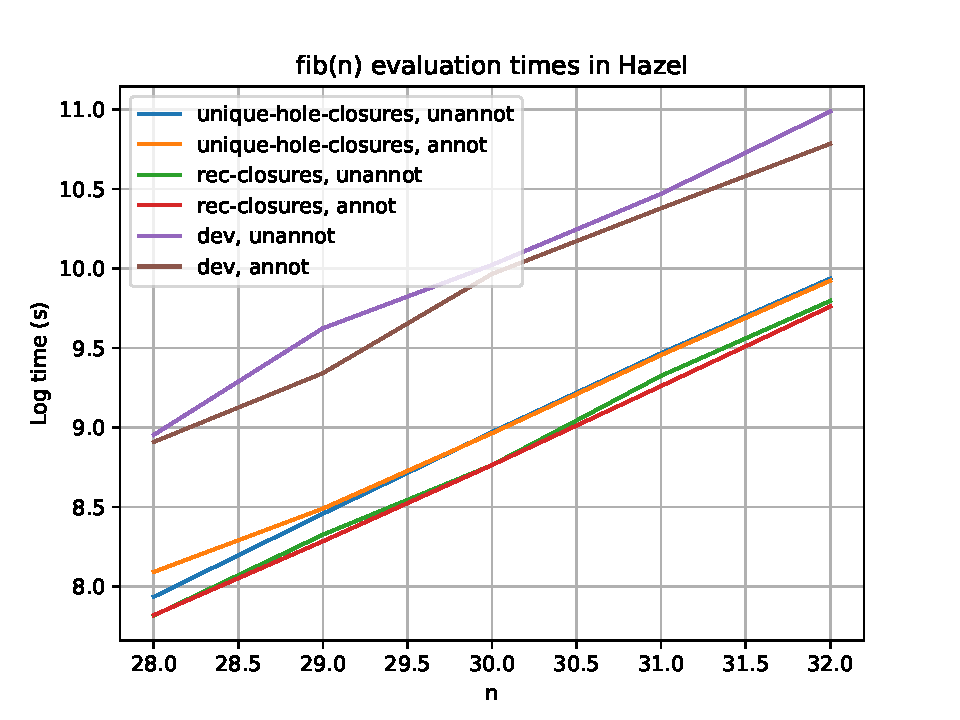
\includegraphics[width=10cm]{img/subst_evalenv_fib_perf.pdf}
  \caption{Performance of the different models of evaluation}
  \label{fig:perf_evaluation_models}
\end{figure}

% TODO: evaluate performance of the above, which has no holes or pseudo-holes
% (is complete (is this the right usage of the word "complete"?) and has no
% possible match failures); show graph of n vs time

% TODO: show a different example and show breakdown of times:
% - evaluation
% - renumbering
% - structural checking
% - (calling evaluate multiple times?)
% - (with and without memoization?)

% TODO: demonstrate fill-and-resume performance improvement

% TODO: evaluation of correctness:
% - fuzz testing and other empirical testing
% - mechanization in Agda (for future work)
% - metatheorems and intuition

%%% Local Variables:
%%% mode: latex
%%% TeX-master: "main"
%%% End:
